\documentclass{bioinfo}

\usepackage{natbib}
\usepackage{multirow}
\usepackage{rotating}
\usepackage{tabularx}
\usepackage{color}

\renewcommand{\multirowsetup}{\centering}
\newcommand{\argmax}[1]{\underset{#1}{\operatorname{arg}\,\operatorname{max}}\;}
\copyrightyear{2005}
\pubyear{2013}

\begin{document}
\firstpage{1}

\title[Detection of Active TFBSs with the Combination of DNase Hypersensitivity and Histone Modifications]
{Detection of Active Transcription Factor Binding Sites with the Combination of DNase Hypersensitivity and Histone Modifications}
\author[Gusm\~{a}o \textit{et~al}]{Eduardo G. Gusm\~{a}o\,$^{1}$, Christoph Dieterich\,$^{2}$, Martin Zenke\,$^{3,4}$ and Ivan G. Costa\,$^{1,5,6,}$\footnote{to whom correspondence should be addressed}}
\address{$^{1}$IZKF Computational Biology Research Group, Institute for Biomedical Engineering, RWTH Aachen University Medical School, Germany.\\
$^{2}$Computational RNA Biology and Ageing, Max Planck Institute for Biology of Ageing, Germany. \\
$^{3}$Department of Cell Biology, Institute for Biomedical Engineering, RWTH
Aachen University Medical School, Germany. \\
$^{4}$Helmholtz Institute for Biomedical Engineering, RWTH Aachen University, Germany. \\
$^{5}$Aachen Institute for Advanced Study in Computational Engineering Science (AICES), RWTH Aachen University, Germany. \\
$^{6}$Center of Informatics, Federal University of Pernambuco, Brazil.
}

\history{Received on XXXXX; revised on XXXXX; accepted on XXXXX}

\editor{Associate Editor: XXXXXXX}

\maketitle

\begin{abstract}

\section{Motivation:} The identification of active transcriptional regulatory elements
is crucial to understand regulatory networks driving cellular processes such as cell
development and the onset of diseases. It has recently been shown that chromatin structure
information, such as DNase I hypersensitivity or histone modifications, significantly
improves cell-specific predictions of transcription factor binding sites. However, no
method have so far successfully combined both DNase I hypersensitivity and histone
modification data to perform active binding site prediction. 

\section{Results:} We propose here a method based on hidden Markov models to integrate
DNase I hypersensitivity and histone modifications occupancy for the detection of open
chromatin regions and active binding sites. We have created a framework which includes
treatment of genomic signals, model training and genome-wide application. In a comparative
analysis, our method obtained a good trade-off between sensitivity vs. specificity and
superior area under the curve statistics than competing methods. Moreover, our technique
does not require further training or sequence information in order to generate binding
location predictions. Therefore, the method can be easily applied on new cell types and
allow flexible downstream analysis such as \emph{de novo} motif finding.

\section{Availability:} Our framework is available as part of the Regulatory Genomics Toolbox.
The software information and all benchmarking data is available at
\href{http://costalab.org/wp/dh-hmm}{http://costalab.org/wp/dh-hmm}.
\section{Contact:} \href{ivan.costa@rwth-aachen.de}{ivan.costa@rwth-aachen.de},\\*
\href{eduardo.gusmao@rwth-aachen.de}{eduardo.gusmao@rwth-aachen.de}
\end{abstract}

\section{Introduction}
\label{sec:introduction}

Transcriptional regulation orchestrates the proper temporal and spatial
expression of genes~\citep{maston2006}. The identification of transcriptional
regulatory elements, such as transcription factor binding sites (TFBSs),
is crucial to understand regulatory networks driving cellular processes
such as cell development and the onset of diseases. The standard approach
is the use of sequence-based bioinformatics methods, which search over the
genome for motif-predicted binding sites (MPBSs) representing the DNA binding
sequence of a transcription factor (TF)~\citep{stormo2000}. This binding
affinity is usually represented by models such as position weight matrices (PWMs).
However, motifs are generally short and have low information content.
Moreover, the presence of a sequence motif does not imply actual TF binding
in that particular cell type. As a result, sequence-based methods return myriads
of putative TFBSs, of which only a small fraction is functional in a particular
context~\citep{maston2006}.

Chromatin immunoprecipitation followed by sequencing (ChIP-seq) allows the
detection of TFBSs \emph{in vivo} on a genome-wide level~\citep{landt2012}.
However, success of ChIP-seq assays depends on the existence of a good antibody
against the TFs of interest and on the availability of large numbers of cells.
These two conditions are not always met in particular for primary cells.
Therefore, ChIP-seq based studies are restricted to the analysis of a small
selection of TFs and cell types~\citep{kim2008,ouyang2009}
or require the effort of large consortia~\citep{encode2012}.

Another solution is to explore the fact that an `open' chromatin structure
is crucial and a prerequisite to the cell type-specific binding of a TF to
DNA~\citep{arvey2012,thurman2012}. For example, regions with histone
modification marks H3K4me3 and H3K4me1 highlight active promoter and enhancer
{\color{red} elements}~\citep{bell2011}. More detailed studies have demonstrated that
active TFBSs occur between two regions with high active histone marks
(peak-dip-peak pattern)~\citep{hon2009}. A classical
method to detect active regulatory elements, DNase I footprinting, has
also been recently combined with sequencing to indicate open chromatin
regions on a genome-wide scale~\citep{crawford2006b}.
DNase-seq allows the identification of putative active TFBSs at
base pair level resolution, i.e. 5--20 bp regions within two DNase-seq
peaks represent the so-called footprints, where TFs are likely to be
bound. While DNase-seq returns the exact position where DNA was nicked by
DNase I enzyme, ChIP-seq returns sequences centered on the protein
interacting with DNA. Therefore, DNase-seq gives a more precise estimate
of open chromatin than histone modification ChIP-seq, as reflected in the
sharpness of the signal of DNase-seq in comparison to H3K4me3 ChIP-seq signal
(see Fig.~\ref{fig:hmm}A). A recent evaluation of DNase-seq on over 50 cell types
indicated that DNase I digestion patterns describe the topology of protein--DNA binding
interfaces and allowed the finding of 394 novel motifs~\citep{neph2012a}.

Several computational approaches explore open chromatin evidence from ChIP-seq
data or DNase I hypersensitivity (DHS) sites to restrict the search space of sequence-based
analysis~\citep{boyle2011,cuellar2012,gusmao2012,natarajan2012,neph2012a,pique2011,whitington2009,won2010}.
They show a clear advantage in detecting active TFBSs, as indicated by ChIP-seq
evidence, in comparison to pure sequence-based methods.

\begin{figure*}[t]
\centering
     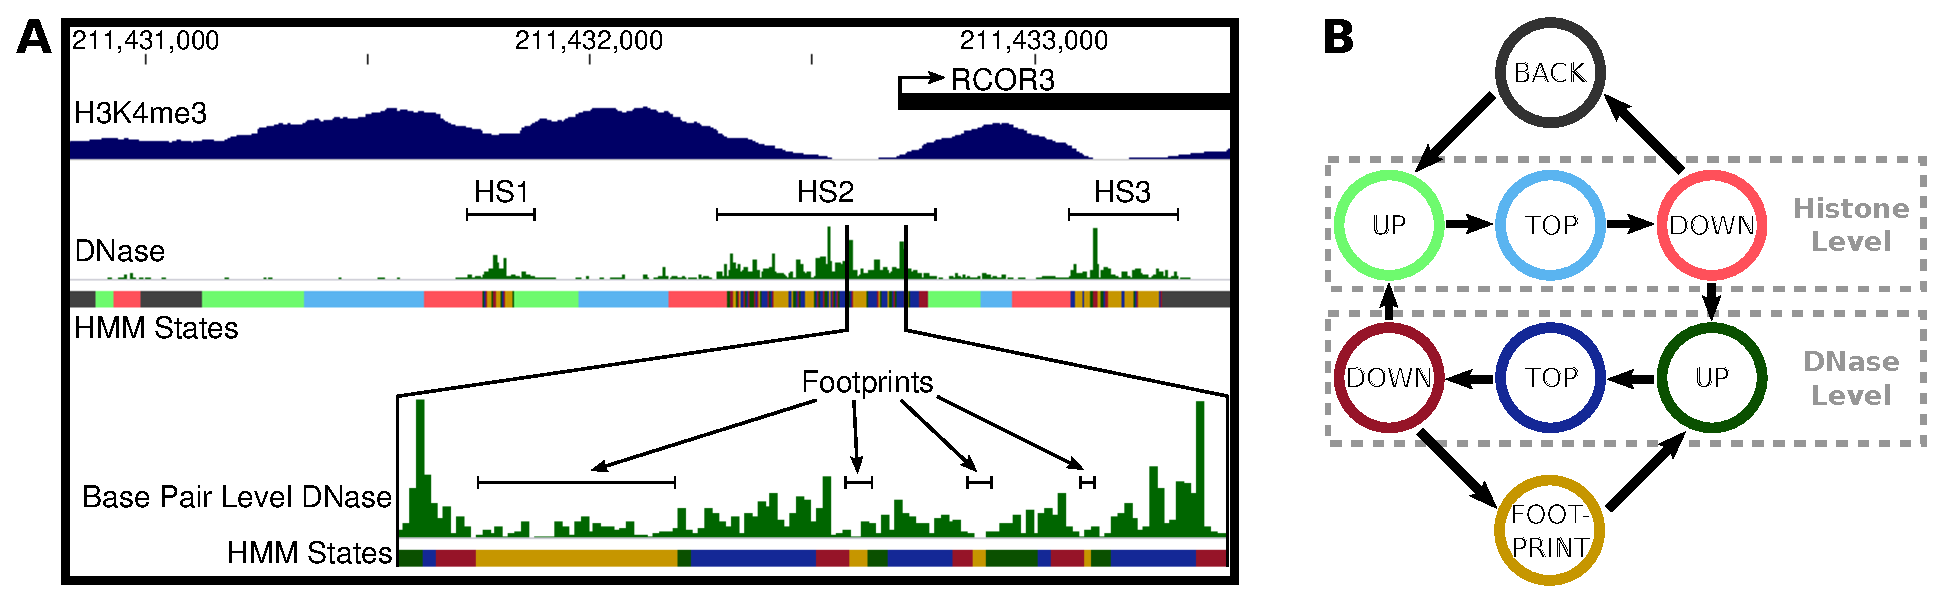
\includegraphics[width=0.99\textwidth]{FootprintsHMM.eps}
%     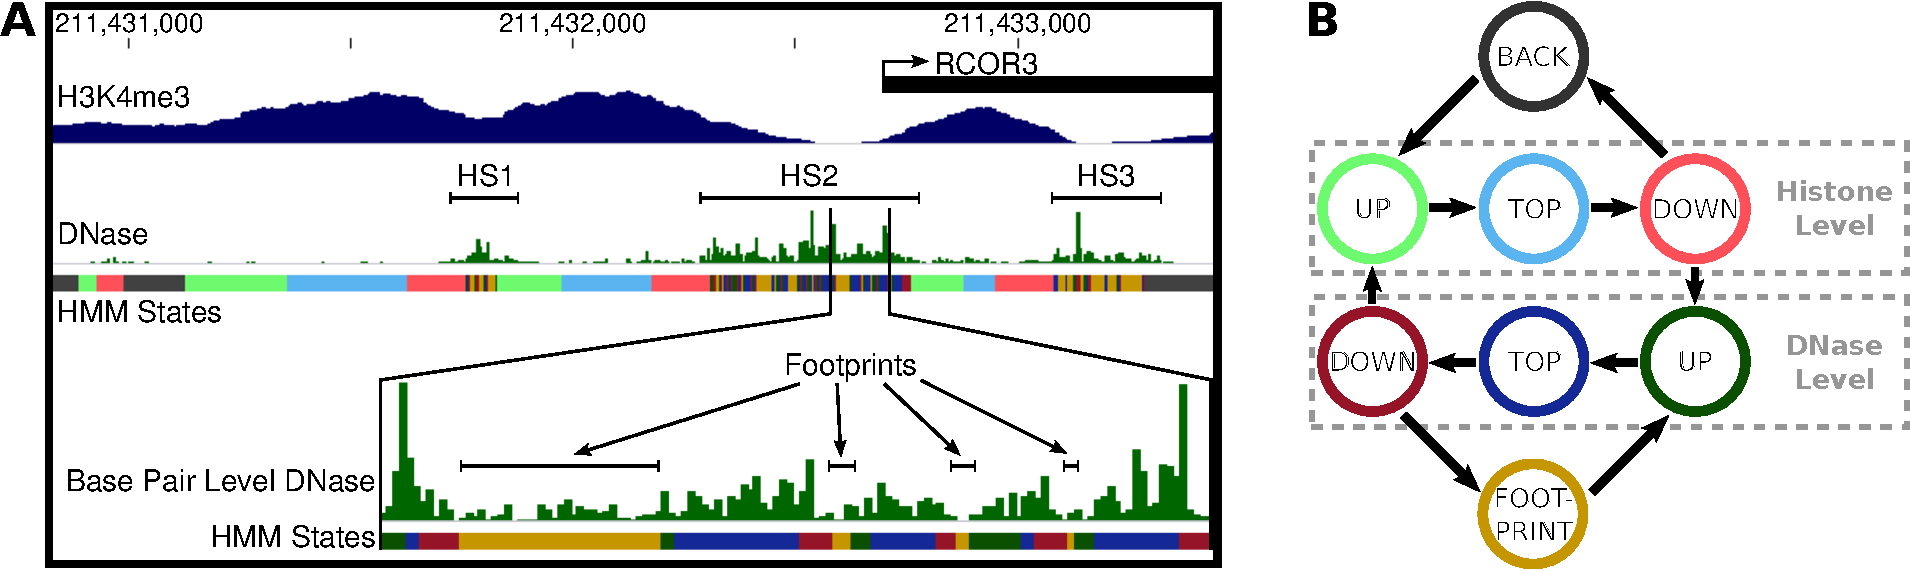
\includegraphics[width=0.99\textwidth]{Figs/FootprintsHMM.pdf}
\caption{Epigenetic grammar. (\textbf{A}) DHS (DNase-seq) and H3K4me3 (ChIP-seq) profiles around the promoter region of RCOR3 -- REST corepressor 3 on K562 cell type. The DNase-seq signal indicates three clear regions of DHS (HS1, HS2 and HS3), each of which fits dip regions within the H3K4me3 signal. Moreover, these regions consist of several putative footprints of varied sizes. (\textbf{B}) Eight state HMM proposed. The first state models background signal ({\tt BACK}). From the background state, the only possible transition is to the histone level states, which will model the increase ({\tt UP}), high levels ({\tt TOP}) and decrease ({\tt DOWN}) of histone modifications. After visiting histone level states, the HMM allows transitions to the DNase level states, which again model the increase, high levels and decrease in the DHS signal. Only then, the {\tt FOOTPRINT} state can be visited. After a footprint visit, the HMM has to go again to the DNase and histone level states, emphasizing the peak-dip-peak pattern. We omit the self-transitions, which are present in all states, for simplicity.}
\label{fig:hmm}
\end{figure*}

\subsection{Previous Approaches}
\label{sec:previous.approaches}

Previous approaches can be categorized in two distinct classes: segmentation-based
methods and site-centric methods. Segmentation-based methods such as~\cite{boyle2011,neph2012a,won2010},
were based on the application of hidden Markov models (HMMs) or sliding window methods
to segment the genome into open (and {\color{red} closed}) chromatin region. \cite{won2010}, for
example, was based on the detection of typical peak-dip-peak profiles of H3K4me3
and H3K4me1 histone modifications indicative of active promoter and enhancer regions.
Afterwards, \cite{boyle2011} proposed an HMM model to detect open chromatin/footprints
in DHS signals on a base pair resolution. Lastly, \cite{neph2012a} applies a
simple sliding window approach that finds small regions (6--40 bp) with low DHS counts
in the middle of regions (3--10 bp) with high DHS counts. Site-centric methods, on
the other hand, perform predictions around MPBSs. For example,~\cite{pique2011}
first detects MPBSs then it applies an unsupervised learning method that uses chromatin
information to group sites as active or inactive. This Bayesian method combines DHS
profiles and histone modification summary statistics around the TFBSs with priors derived
from motif matching bit-score, sequence conservation and distance to the nearest transcription start site.
Later, \cite{cuellar2012} improved the methodology proposed in~\cite{whitington2009} to
include the combination of DHS and distinct histone modification as priors in the detection
of active MPBSs. They showed that DHS improves TFBS detection considerably. Nevertheless,
no significant improvement was observed when DHS was combined with histone modifications.
Interestingly, \cite{pique2011} also could not observe advantages in using histone
modifications. Note, however, that both ~\cite{pique2011} and \cite{cuellar2012} use simple
window-based statistics for histone modification, which are unable to detect peak-dip-peak
shapes as in~\cite{won2010}.

\subsection{Our Approach}
\label{sec:our.approach}

We propose here an HMM-based approach to integrate both DHS (DNase-seq) and histone
modifications (ChIP-seq) for the detection of open chromatin regions and active TFBSs.
We and others have previously observed that the peak-dip-peak patterns of the DHS
profile happen inside the dip of the histone modification profiles~\citep{gusmao2012,kundaje2012}
(see Fig.~\ref{fig:hmm}A). This indicates an underlying epigenetic grammar
behind active TFBSs: open chromatin regions (high DHS) are flanked
by high or moderate signals of active histone marks. These open chromatin regions
consist of a sequence of one or more footprints indicative of active TFBSs (low histone
modification and DHS signals). We have therefore devised an HMM (Fig.~\ref{fig:hmm}B)
to model this epigenetic grammar by simultaneous analysis of DNase-seq and the ChIP-seq
profiles of the histone marks H3K4me1, H3K4me3, H3K9ac, H3K27ac and H2A.Z, which are
indicative of active regulatory regions, on a genome-wide level. The HMM has as input
a normalized and a slope signal of DHS and one histone mark. It can therefore
detect the increase, top and decrease regions of both histone mark and DHS signals.
The HMM has multivariate Gaussian density functions with full covariance matrices as
emission functions in order to capture correlations between the DHS and histone
marks signals. As in~\cite{boyle2011}, we trained the HMM on the annotation of a single
genomic region. Moreover, we devised a normalization procedure of the DHS/histone mark
profiles to allow the application of an HMM trained in a particular cell type to be
applied on any cell type of interest. This is the first approach combining local genomic
profiles of histone modification and DHS for the detection of open chromatin and active
TFBSs. We evaluate our and competing methods with public data from H1-hESC and K562
cell types. To validate our predictions, we created datasets by combining MPBSs with
ChIP-seq from 83 TFs.

\begin{methods}
\section{Method}
\label{sec:method}

\subsection{Epigenetic Signal Processing}
\label{sec:signal.processing}

Let the matrix~$\mathbf{X}$ representing genomic signals be defined as
\begin{align*}
    \mathbf{X} = {\{{x}_{ij}\}}^{D \times N},
\end{align*}
where~$ D $ is the number of genomic signals and~$N$ refers to the
number of bases in the genome. The $i$th genomic signal is
represented by the vector
\begin{align*}
    \mathbf{{x}_{i\cdot}} = \{{x}_{i1},...,{x}_{iN}\}.
\end{align*}
and the genomic signals at the $j$th position are represented as 
\begin{align*}
    \mathbf{{x}_{\cdot j}} = \{{x}_{1j},...,{x}_{Dj}\}.
\end{align*}

The first processing step consists on creating a base-pair resolution
genomic coverage signal by counting the reads mapped to the genome.
For DHS data, we only consider the first 5$^\prime$ position of
the aligned reads (corresponding to the exact position at which DNase
I enzyme has nicked the DNA). For histone modification ChIP-seq data,
we extend all the aligned {\color{red} reads to be 200 bp long}, as this is the
expected length of immunoprecipitated fragments. Then, in both cases,
the resulting genomic signal is created by counting how many
reads overlapped at each genomic position.

The signals are then normalized using an approach that addresses both
within- and between-dataset variability. For that, the genome is
partitioned into a set $\{b_1,...,b_M\} $ of non-overlapping bins
and a set $\{r_1,...,r_M\} $ of overlapping bins.
Each bin $b_m$ covers the genomic coordinate interval $[((m-1) \cdot L )+1,m \cdot L]$,
and $r_m$ represents $b_m$ extended by $L/2$ for both sides. 
By using $L=5000$, we partition the genome in regions with total
length $10000$. First, we apply a within-signal
normalization by averaging non-zero read counts inside bins~\citep{boyle2011}.
For a given position $x_{ij}$, such that $j \in b_m$, we apply
\begin{align}
    x^{{norm1}}_{ij} = \frac{x_{ij}}{ 
                        \sum\limits_{w \in {r_m}} x_{iw} \mathbf{1}({x}_{iw}>0)  \;\; \Big/  
                        \sum\limits_{w \in {r_m}} \mathbf{1}(x_{iw}>0)
                        },
    \label{eq:norm1}
\end{align}
where $ {\mathbf{1}}(\cdot) $ denotes the indicator
function. Next, we perform a between-dataset scaling procedure
following~\citep{hon2009} to force values inside the interval $ [0,1] $.
Assuming $j \in b_m$, this is done by applying a logistic function
to the first normalized values as follows
\begin{align}
    {x}^{{norm2}}_{ij} = \frac{1}{1+e^{{-(x^{{norm1}}_{ij}-P^{t}_{r_m})}/{\sigma}_{{r_m}}}},
    \label{eq:norm2}
\end{align}
where $\sigma_{r_m} = \sqrt{ \sum_{w \in r_m} (x_{iw} - \mu_{r_m})^2/(2L) }$,

\noindent
$\mu_{r_m}=  \sum_{w \in r_m}  x^{norm1}_{iw}/(2L)$  and $P^{t}_{r_m}$ are, respectively, the standard deviation, mean and the $t$th percentile of values $x^{norm1}_{iw} \in r_m$.

In order to estimate the slope of the signals we apply a Savitzky-Golay
smoothing filter. This method consists of fitting the data into
a 2nd order polynomial, performing a convolution (based on a specific
window length) with a vector containing Savitzky-Golay
coefficients~\citep{madden1978}. The window length was set to 9 bp
(including the central element) for DHS data~\citep{boyle2011}
and 201 bp for histone modification ChIP-seq data, matching the read
extension length. Next, the first derivative is applied to the
smoothed signal. The resulting signal represents the slope of the
normalized curve and assumes positive values when there is an increase
and negative values when there is a decrease. The slope signal will
help the delineation of the start and end of DHS and histone
modification peaks (see Supplementary Fig.~2 for examples of these signals).

\subsection{Prediction of footprints with HMMs}
\label{sec:prediction.footprints}

The HMM structure was designed to recognize the epigenetic grammar
described in Section~\ref{sec:our.approach}. This segmentation task is
performed based on four input signals: the normalized and slope versions
of both DHS and a histone modification. The structure,
depicted in Fig.~\ref{fig:hmm}B can be interpreted as follows.
The first state ({\tt BACK}) corresponds to the `background' regions
with low concentration of DHS and histone marks. The
histone level states represent a peak in the histone modification signal,
recognizing an increase in the histone modification signal based on high positive
slope values ({\tt UP}), summit regions with slope
values close to zero with high normalized values ({\tt TOP}) and a
decrease based on negative values of the slope signal ({\tt DOWN}).
From the histone level {\tt DOWN} state, the model can either return
to {\tt BACK} (isolated histone modification peaks without further DHS) or continue
to the DNase level {\tt UP} state. The DNase
level states are equivalent to the histone level states, with the
exception that the DHS normalized and slope signals are being
recognized instead. From the DNase level {\tt DOWN} state, the model
decides between returning to a region of higher histone
modification signals (histone level {\tt UP} state) and visiting the
{\tt FOOTPRINT} state, which represents the dip between two peaks of
intense DHS. The regions of the genome where the HMM has
recognized as {\tt FOOTPRINT} are the ones reported by our method as
likely TFBSs. See Supplementary Section~3.3 for alternative HMM topologies.

More formally, for an observed multivariate sequence $\mathbf{X}$ and
a hidden variable $\mathbf{Q}=\{q_1,...,q_N\}$, we can describe an HMM
by parameters $\Theta= A,B,\Pi\}$. $A$ represents the state
transition matrix
\begin{align*}
    A = {\{a_{uv}\}}^{S \times S},
\end{align*}
where~$S$ is the number of states and $a_{uv}$ represents the
probability of transition from state $u$ to $v$. The initial state
transition probabilities are represented as
\begin{align*}
    \Pi = \{\pi_{1},...,\pi_{S}\}.
\end{align*}
We use a multivariate normal density function with full covariance matrix as emission probability
of the states. For a given genomic position $j$ and state $u$ we have
\begin{align}
    \begin{array}{lcl}
p(\mathbf{x_{\cdot j}}|q_j=u) & = & p(\mathbf{x_{\cdot j}}|{{\mu}^{u}},{{\Sigma}^{u}})\\[0.4em]
                          & = &
\frac{1}{ \sqrt{(2\pi)^{D} {| {{{\Sigma}^{u}}} |}}}
e^{-\frac{1}{2} (\mathbf{x_{\cdot j}}-\mu^u)^T (\Sigma^u)^{-1} (\mathbf{x_{\cdot j}}-\mu^u)}, \\
    \end{array}
    \label{eq:gaussian}
\end{align}
where $\mu^u$ and $\Sigma^u$ are respectively the $D$-dimensional
mean vector and full covariance matrix. Lastly, the emission parameters $B$ are
defined as $\{(\mu^1,\Sigma^1),...,(\mu^S,\Sigma^S)\}$.

\subsubsection{Model Training and Decoding}
\label{sec:hmm.training}

The HMM is trained with maximum likelihood parameters on a supervised
approach. For a given annotation sequence of the hidden data $\mathbf{Q}$ and
sample data $\mathbf{X}$, the parameters are estimated as
\begin{align}
    a_{uv} = \frac{ \alpha^{\prime}_{uv}}{ \sum_{w=1}^{S} \alpha^{\prime}_{uw}},
    \label{eq:train1}
\end{align}
where $\alpha^{\prime}_{uv}=\sum_i^{N-1} \mathbf{1} (q_i=u,q_{i+1}=v)$
represents the number of transitions from state~$u$ to state~$v$
observed in the training data. 

As we expect the HMM to always start at the {\tt BACK} state, the initial
transition vector $\pi_1=1$ and $\pi_u=0$ for $u > 1$. 

Finally, the emission parameters are estimated as
\begin{align}
\mu^{u} = \frac{ \sum_{j=1}^{N} {x}_{\cdot j} {\mathbf{1}}(q_j=u) }{ \sum_{j=1}^{N} {\mathbf{1}} (q_j=u) },
    \label{eq:train2}
\end{align}
and
\begin{align}
    {\Sigma}^{u} =  \frac{ \sum_{j=1}^{N} ({x}_{\cdot j} - {\mu}^{u})^T({x}_{\cdot j} - {\mu}^{u}) {\mathbf{1}} (q_j=u)}
                         { \sum_{j=1}^{N} {\mathbf{1}} (q_j=u)  - 1}.
    \label{eq:train3}
\end{align}

The final goal of our model is to find the most probable states
visited for a given genomic signal. More formally, we want to find the
most probable sequence of hidden states $ \mathbf{Q}$ having
observed~$\mathbf{X}$ given a model~$ \Theta$, which can be written as
\begin{align}
    \mathbf{Q^*} = \argmax{\mathbf{Q}} p\left(\mathbf{X},\mathbf{Q}|\Theta\right).
    \label{eq:viterbi1}
\end{align}
The solution to the above problem is given by the Viterbi algorithm~\citep{rabiner1989}.
In practical terms, we consider positions annotated with the {\tt FOOTPRINT}
state to be potential active TFBSs.

\section{Experimental Design}
\label{sec:experimental.design}

\subsection{Datasets}
\label{sec:datasets}

Both DNase-seq and ChIP-seq for TFs and histone modifications data were obtained
in ENCODE repository~\citep{encode2012}. We used read alignments available for
the embryonic stem cell (H1-hESC) and myelogenous leukemia (K562). DNase-seq and
ChIP-seq for H3K4me1, H3K4me3, H3K9ac, H3K27ac and H2A.Z were downloaded for every
cell type in order to generate the input for the HMMs (see Supplementary {\color{red} Table~22}
for details on input data).

In order to create the evaluation dataset, we obtained all ChIP-seq enriched
regions for TFs of these two cell types in ENCODE Analysis Working Group (AWG) data track.
Also, we used PWMs from Jaspar~\citep{mathelier2014}, Transfac~\citep{matys2006}
and Uniproble~\citep{robasky2011} repositories (see Supplementary {\color{red} Tables~23--25}
for details on evaluation data).

All experimental files and alignments are based on the human genome build 37 (hg19).
Chromosome Y has been removed from all analyses.

\subsection{HMM Training and Evaluation}
\label{sec:application.hmm}

To reduce the dimensionality of the data, we first applied a peak calling tool
to find regions with evidence of DHS and histone modification signals. The enriched
regions of histone modifications ChIP-seq data were defined using the peak-calling
tool MACS~\citep{zhang2008}. We used a $p$-value of $ 10^{-5} $ and all default
parameters from MACS 1.4. No further filtering, such as false discovery rate, was
performed on the peaks, as we wanted a lenient selection of candidate regions. The
enriched regions of the DHS data were defined as in~\cite{boyle2011}. Briefly, a
signal corresponding to the estimated density of the DHS is generated by applying F-seq
software~\citep{boyle2008b} to the DNase-seq mapped reads and background information
based on alignability, copy number and karyotype correction. A threshold is then
calculated by fitting the signal to a gamma distribution and considering the value
that corresponds to a loose $p$-value of $ 0.01 $. We merge all enriched regions
for a given cell type and extend them by 5000 bp in each direction. This step keeps
only $3-6\%$ of the genome with DHS or histone modification evidence for a given
cell type (see Supplementary Table~5 for complete statistics).

We selected a 10,000 bp region around the promoter of the gene RCOR3 and performed
a cell type-specific manual annotation with one of the 8 HMM states according to the
epigenetic grammar described in Fig.~\ref{fig:hmm}. As one of the histones marks
-- H3K4me1 -- is known to be associated to distal enhancers, we have additionally
annotated an enhancer region. The selection of these regions was made randomly, but
we checked ENCODE tracks for evidence that the gene RCOR3 was expressed in all cell types
analyzed and that the enhancer region was far ($>$100kb) from known genes and expressed
regions.

In order to help the annotation of the footprints, MPBSs with all PWMs from Jaspar,
Transfac and Uniprobe datasets were detected inside the training regions. We consider
(active) footprints all the signal depleted regions between two DHS peaks that overlap
a MPBS. We trained five HMMs per cell type, one for each histone modification (H3K4me3, H3K9ac,
H3K29ac and H2A.Z with the promoter region and H3K4me1 with the enhancer region). The regions
used for training were excluded from all further predictions. We used the Viterbi algorithm
to find the footprint regions throughout the genome for each trained HMM. Note that the
evaluation of the HMM on the genomic signals was performed regardless of any evidence that
the regions are distal/proximal to a gene. See Supplementary Section~3.1 for details
on training and Supplementary Tables~2--4 for the set of parameters for the HMM trained
using DHS+H3K4me3 on H1-hESC data.

\subsection{Evaluation}
\label{sec:evaluation}

\subsubsection{Binding Evidence}
\label{sec:sequence.evidence}

ChIP-seq experiments for the TFs being tested were used as experimental evidence of binding.
These are simply the enriched regions (or peaks) based on the uniform processing of ENCODE
Analysis Working Group (AWG) data track. Next, we used the \emph{de novo} motif analysis
from Factorbook~\citep{wang2013} to select the PWMs associated with the TF ChIP-seq data.
We considered only the TFs in which the top enriched motif was present in at least $300$ of
the $500$ top-scored ChIP-seq peaks. We used PWMs from the Jaspar database matching those
in Factorbook. Four PWMs (ATF1, BACH1, NR2F2 and SP4) not present in Jaspar were obtained
from Transfac and Uniprobre.

These PWMs were matched against the complete human genome using the motif matching tool
available in Biopython~\citep{cock2009}. Initially, a regularizing value of $ 0.05 $ was
added for all nucleotides at all positions of the PWMs. We used a false positive rate (FPR)
($10^{-4}$) approach based on dynamic programming~\citep{wilczynski2009} to detect significant
MPBSs. In this scenario, a different threshold is calculated for each PWM by defining the
bit-score that corresponds to a specific FPR in the distribution of scores of that TF's PWM. Note
that~\cite{pique2011} used a fixed bit-score cutoff of $ log_2(10000) = 13.288 $ for all PWMs.
However, we observed that this criterion is very strict, in the sense that only a few MPBSs
coincide with regions enriched with experimental ChIP-seq data (see Supplementary Section~2.2
for discussion). Finally, we filtered out all TFs in which less than $10\%$ of ChIP-seq peaks
contained at least one MPBS associated. This resulted in a set of 56 TFs from K562 and 27 TFs
for H1-hESC cell types (see Supplementary {\color{red} Tables~23--25} for the final selection of PWMs and TFs).

\subsubsection{Gold Standard and Evaluation Metrics}
\label{sec:gold.standard}

To evaluate all methods, a site-centric gold standard was proposed~\citep{cuellar2012}.
In this evaluation scheme MPBSs with ChIP-seq evidence (i.e. lying within 100 bp from
the peak summit) are considered `true' TFBSs and all other MPBSs are considered `false'
TFBSs. Then, every footprint prediction that overlaps by at least 1 bp with a true TFBS
is considered a correct prediction (true positive -- TP) {\color{red} and every footprint
that overlaps with a false TFBS is considered an incorrect prediction (false positive -- FP).}
Consequently, true negatives (TN) and false negatives (FN) are, respectively, {\color{red}
false and true TFBSs without overlapping footprint predictions.}
{\color{red} With such contingency
table we are able to calculate the sensitivity and specificity of each method}. In Supplementary {\color{red} Tables~17--19}
we show statistics on the number of MPBSs, ChIP-seq peaks and combinations of both.

To access the sensitivity $TP/(TP+FN)$ vs. specificity
$TN/(TN+FP)$ trade-off we created receiver operating characteristic
({\color{red} ROC-like}) curves (with true negative rate (specificity) on x-axis, instead of the traditional
false positive rate) and estimated the area under the {\color{red} ROC-like} curves (AUCs) as follows. For each
method, the MPBSs from the gold standard were divided into two groups: the ones that contain
at least 1 bp overlap with the predicted sites and the ones that do not overlap. Both groups
were sorted based on the motif matching bit-score. A single list is then obtained by combining
the ranked list of predicted sites before the ranked list of the non-predicted sites. A {\color{red} ROC-like}
curve was evaluated based on this list, for all cell types and TFs.

\subsection{Competing Methods}
\label{sec:competing.methods}

We compared our method with Boyle method~\citep{boyle2011}, Centipede~\citep{pique2011},
Cuellar-Partida method~\citep{cuellar2012} and Neph method~\citep{neph2012a} using the
evaluation methodology defined previously. Boyle and Neph methods analyses were based on
results/parameterization available in the original studies. As Cuellar-Partida used a
distinct statistical framework for PWM detection, we performed experiments to select the
cutoff criteria. Centipede presented very poor results with default parameters. We have
therefore performed a grid search strategy to detect the best parameterization in one cell
type and applied to the other cell type. This leads to results close to an optimistic
parameterization, where parameter tuning was performed for each TF and cell type combination.
Note that this optimistic parameterization is only possible with ChIP-seq for every TF
tested. Moreover, the estimated parameters from both cell types were similar (level of shrinkage
of negative binomial's parameters was estimated as $0.0$ for H1-hESC and $0.25$ for K562
and level of shrinkage of multinomial's parameters was estimated as $0.75$ for both cell
types) and represent a better choice of default parameters than the ones provided by the
tool. See Supplementary Section~4 for further details on parameterization experiments for
the competing methods. As we could not succeed in running the HMM-based histone segmentation
approach from~\cite{won2010}, we adapted our approach to use only histone modification
signals. For such, the DNase level states were replaced by a
single {\tt FOOTPRINT} state. All the steps described in Section~\ref{sec:application.hmm}
were performed again using new manually annotated regions based on the new HMM state
configuration. This method will be referenced as H-HMM (Histone HMMs). All parameter tuning
experiments were performed on chromosome~1 and these regions were excluded from the method
comparison analysis. All annotations, predictions and evaluation data are available in our
web supplement for future benchmarking purposes.

\subsection{HMM Parameter Selection}

We have performed a set of experiments to evaluate/justify methodological choices for our
approach. For this, we used the genomic signals of chromosome~1, which was left out of any
further analysis. First, we evaluated choices of scaling parameters: use of global or local
statistics in Eq.~\ref{eq:norm2} and value of the percentile (96$\%$, 98$\%$ and 99$\%$).
Results indicate the advantage of local normalization and that 98$\%$ was a good trade-off
between sensitivity and specificity. We have also compared the use of the Viterbi algorithm
and posterior decoding to detect the footprints. Experimental results indicate a slight
advantage of the Viterbi algorithm, while the posterior decoding had numerical problems
in particular genomic regions. We have also evaluated two distinct HMM topologies. The first
alternative merges {\tt UP}--{\tt TOP}--{\tt DOWN} states in one to obtain a simple HMM. This HMM has
very poor performance, as it does not take advantage of the slope of the DHS/histone modification signals.
We have also extended the original HMM topology by including transitions from the background
states directly to the DNase level states. This modification allows the detection of DHS peaks
between asymmetric histone modification signals, which were evidenced in~\cite{kundaje2012}.
The HMM had smaller AUC values than the HMM model proposed here and was therefore not
explored. See Supplementary Section~3 for further discussion regarding all empirical
analyses on HMM parameter selection. All HMMs were implemented using Scikit~\citep{pedregosa2011}.
All experiments were executed in 4 Xeon E7-4870 CPUs with 10 2.4GHz cores each.

\end{methods}

\section{Results}
\label{sec:results}

\subsection{Selection of Histone Modifications}

Given the predictions made by our method (referenced from this point as DH-HMM --
DHS+Histone HMMs) in which different histone modifications are used as input, it is
possible to create combined footprints. Briefly, we take the union of all predictions
from any number of models and merge all overlapping footprints. Then, an initial question
would be the selection of the optimal set of histone marks to be combined. We are particularly
interested in using as few marks as possible to minimize the necessity of high-throughput
experiments. For such, we have evaluated the AUC values of all combinations (up to three)
of the five histone marks on chromosome~1. Results indicate that combinations with more histone marks
are better than single-histone models (see Supplementary Fig.~7 and Table~7). 
Several combinations of three marks (H3K4me1+H3K4me3+H3K9ac, H3K4me1+H3K4me3+H3K27ac, H2A.Z+H3K4me1+H3K4me3,
H2A.Z+H3K4me3+H3K9ac and H3K4me3+H3K9ac+H3K27ac) were similarly good, i.e. their AUC are not
significantly lower than any other combination). Similarly, if we only consider individual
and pairs of histone marks, H3K4me1+H3K4me3, H3K4me3+H3K9ac, H3K4me3+H3K27ac, H2A.Z+H3K4me3 and
H3K4me1+H3K9ac have similar AUCs. This indicates that any combination of these histone marks,
whenever available, would perform equally well. We have selected the combinations
H3K4me1+H3K4me3+H3K9ac and H3K4me1+H3K4me3, which we call DH-HMM(3) and DH-HMM(2),
respectively, for further analysis. We also used the same histone modification selection for all
competing methods that use histone modification evidence (Cuellar(2), Cuellar(3), H-HMM(2) and H-HMM(3)). 
{\color{red} Moreover, we have performed this analysis for
H1-hESC and K562 cell types in separate. Despite small differences in rankings, a similar set of combinations resulted as equally good and both H3K4me1+H3K4me3+H3K9ac and H3K4me1+H3K4me3 were among the top 2 combinations in either cell. See Supplementary Section~3.5 for further discussions.}

\subsection{Cell type specific vs. non-cell type specific training}

Next, we have analyzed if the DH-HMM models are specific for the cell types they are trained
on. In this particular test, we have extended our datasets to include two new cell types
(HeLa-S3 and HepG2) with 20 and 21 TFs, respectively (more details on Supplementary
{\color{red} Tables~20--21 and 26--27}). We have compared the AUC values of the H3K4me1+H3K4me3 DH-HMM
when it was trained in a particular cell type and executed in the same cell type vs. the other
three cell types. A statistical test (paired Mann-Whitney-Wilcoxon with null hypothesis that
the distributions are equal) was performed and showed that only in 1 out of 12 comparisons
the cell type-specific training had significantly superior AUC than a non-specific
training (see Supplementary Section~3.6). This indicates that the DH-HMM models can be
applied to any other cell type data with an insignificant loss of performance.

\subsection{Method Comparison}
\label{sec:prediction.accuracy}

We show in Fig.~\ref{fig:roc} the {\color{red} ROC-like} curves for TFs GABPA, C-jun, SIX5 and YY1 and
cell types H1-hESC and K562.  {\color{red} All methods analyzed provided a list of active TFBSs given a particular parameterization
(see Supplementary Section~4 for details). An exception is Centipede, in which we used
the model's posterior probability to rank sites and the suggested probability ($0.99$)
to select active TFBSs as performed in~\cite{pique2011}. The curves were obtained by ranking the active TFBSs
predictions in regard to the PWM bit-score. To obtain complete curves, we also included
in the end of the ranking the inactive TFBSs (sorted by PWM bit-scores). Squares (and circles) in the
curve indicate the location of the rank with TFBSs predicted to be active only. These points were used to obtain the sensitivity and specificity of a method}.

We tested the ranks of the methods for all 83
combinations of cell types and TFs regarding AUC, sensitivity and specificity. We used the
Friedmann-Nemenyi test to evaluate the statistical significance of the method's ranks.
As indicated in Table~\ref{tab:friedman.nemenyi} and Supplementary Table~1, HMMs
based on histone modification only (H-HMM) had significantly lower values for all indices. This can
be explained by the fact that the histone modification signal, measured by ChIP-seq,
contains a much lower resolution than, for instance, the signal obtained with DNase-seq,
which is used by all other competing methods.

Boyle and Neph methods have significantly higher specificity values than competing
methods {\color{red} (Table~1)}. We observed that, in general, Boyle makes very few predictions,
resulting in very few false positives, but missing many of the true active TFBSs.
For example, from the 3020 observed active GABPA binding sites in H1-hESC, only 2066
(68.41$\%$) and 2207 (73.08$\%$) were detected by Boyle and Neph, respectively; while
Centipede and the DH-HMM(3) predicted 2765 (91.56$\%$) and 2892 (95.76$\%$), respectively.
Indeed, Boyle and Neph methods' sensitivity is significantly lower than all other DHS-based
methods.

The Cuellar method with either 2 or 3 histone modifications presented the highest sensitivity values,
which were statistically higher than all methods but Centipede and DH-HMM(3) {\color{red} (Table~1)}. On the other
hand, Cuellar had very poor specificity values being significantly lower values than all
DHS-based methods. Since the number of false TFBSs is very high, Cuellar usually predicts
a great number of false positives. For instance, Cuellar(3) predicts 5.63$\%$ (10,051 sites)
more false positives than DH-HMM(3) on GABPA binding in H1-hESC. DH-HMM(2) and DH-HMM(3)
significantly outperformed all other methods concerning AUC values (Table~\ref{tab:friedman.nemenyi})
and were significantly better ranked than all other methods in Friedman ranking
(Supplementary Table~1).

\begin{figure*}[t]
\centering
     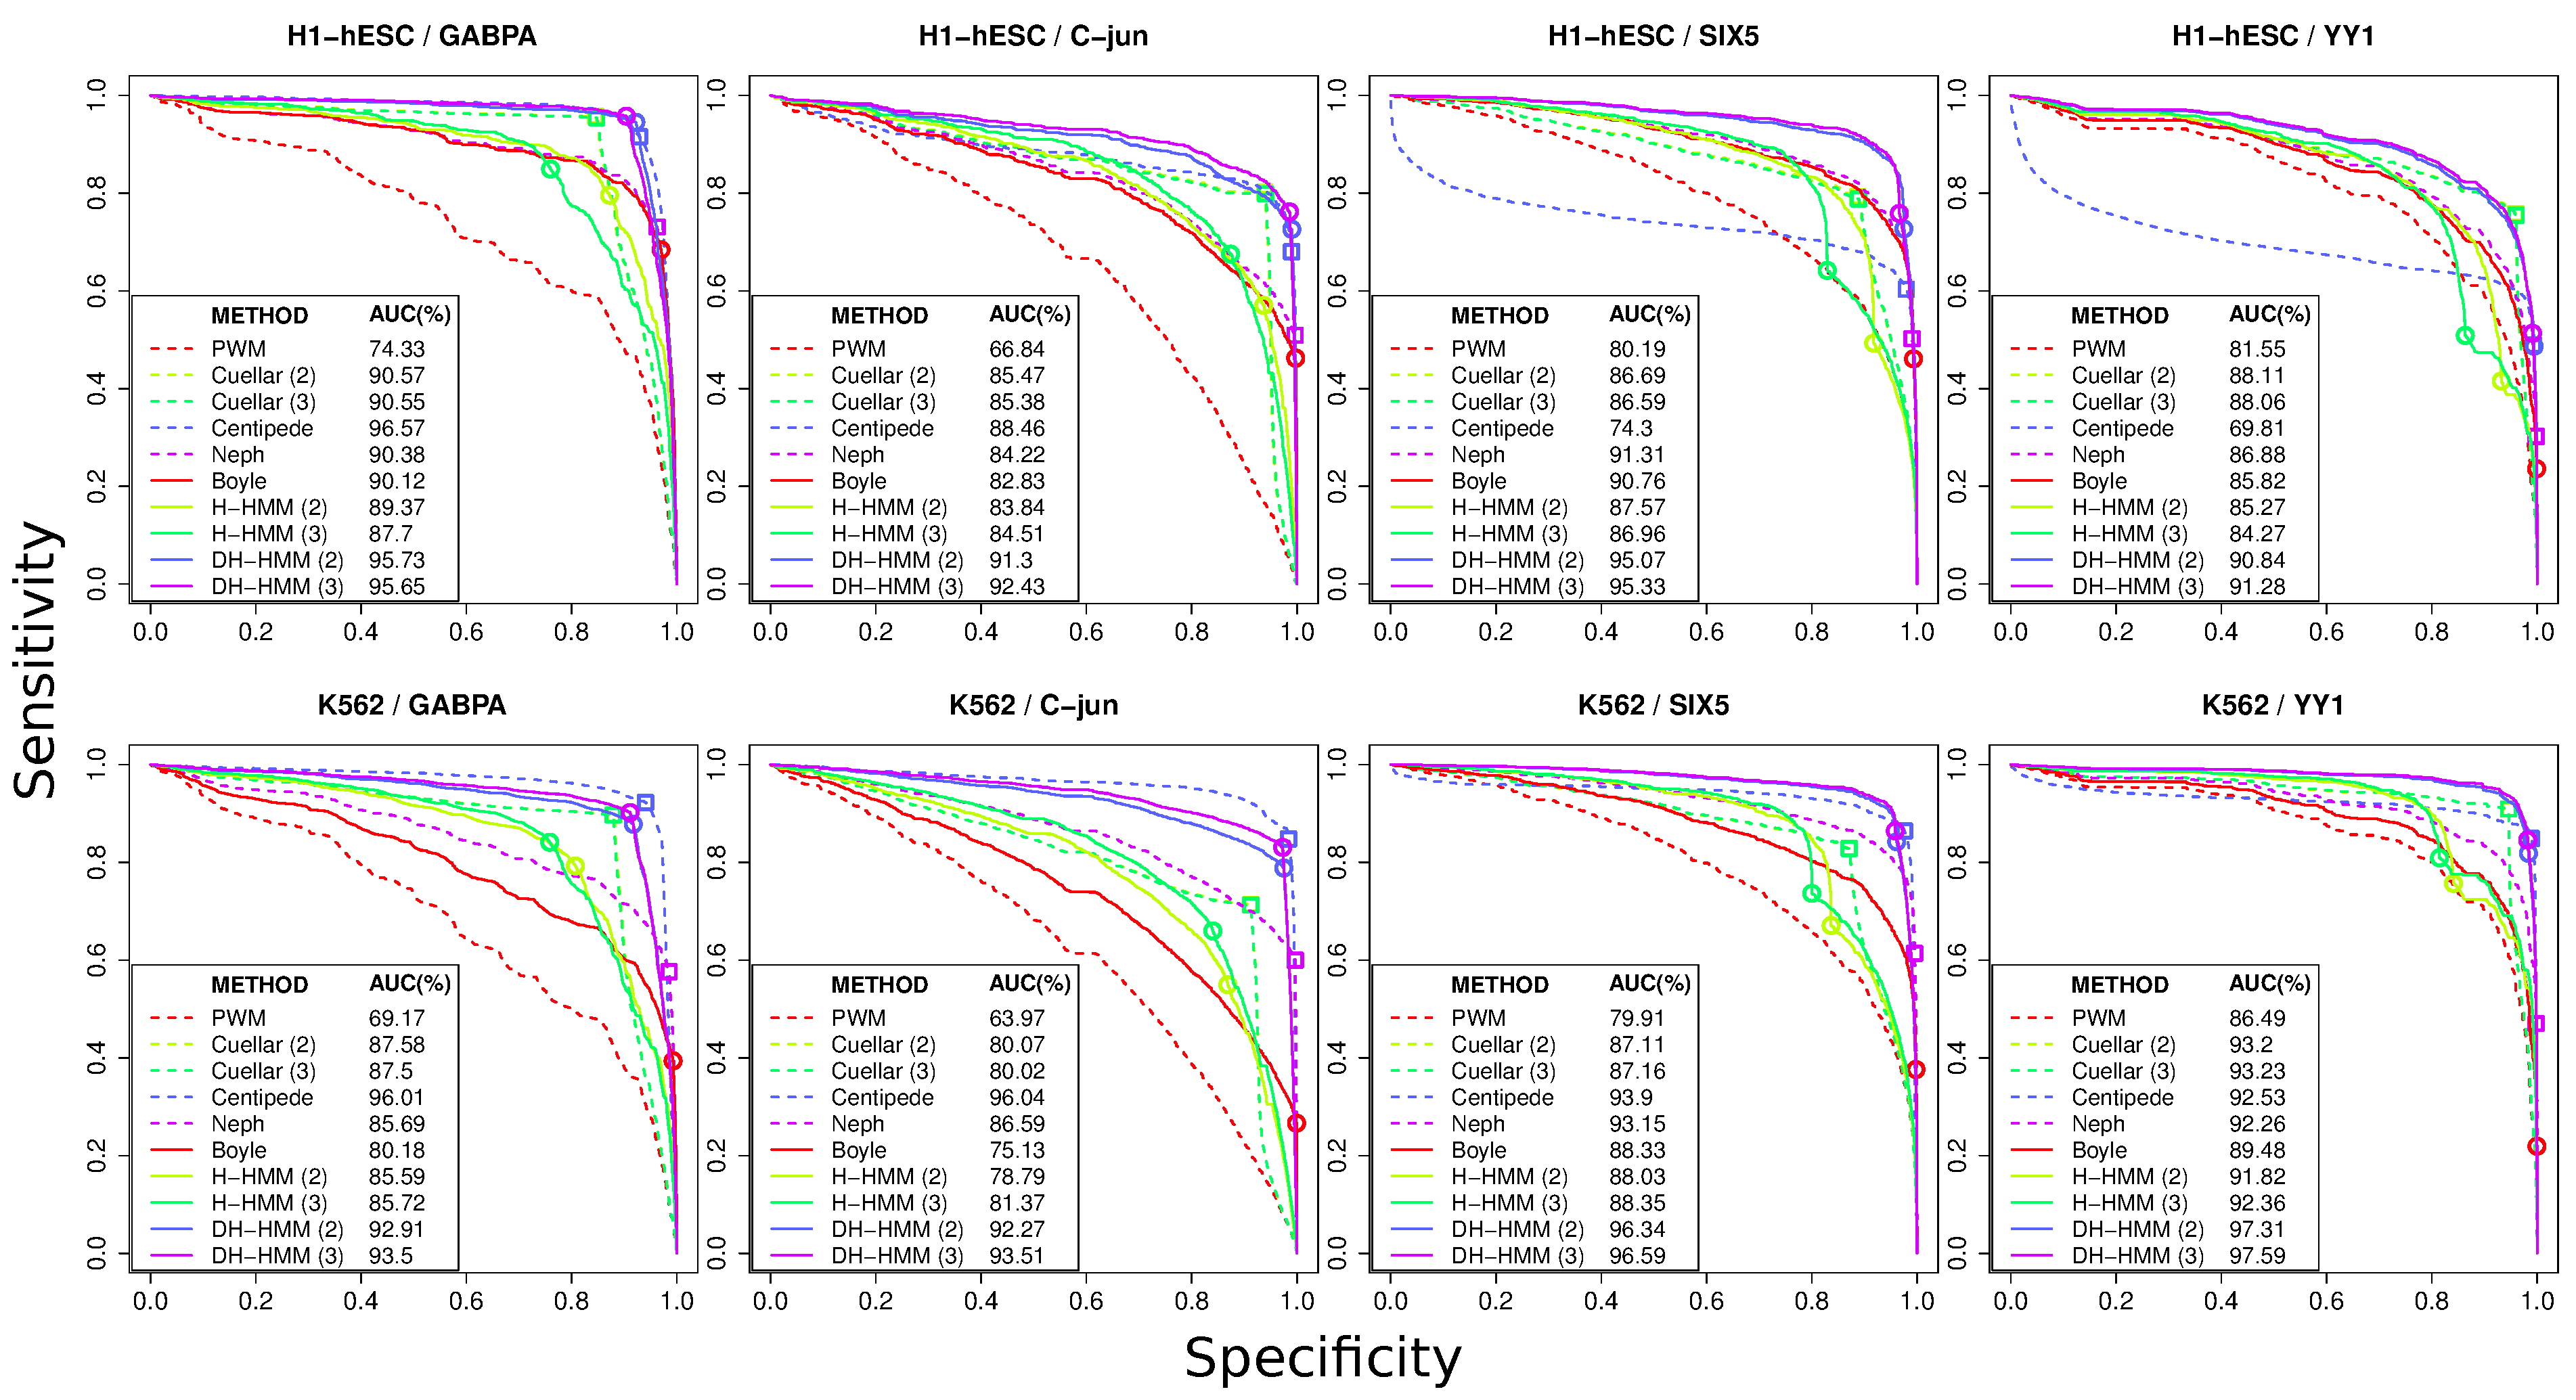
\includegraphics[width=0.99\textwidth]{ROC.eps}
%     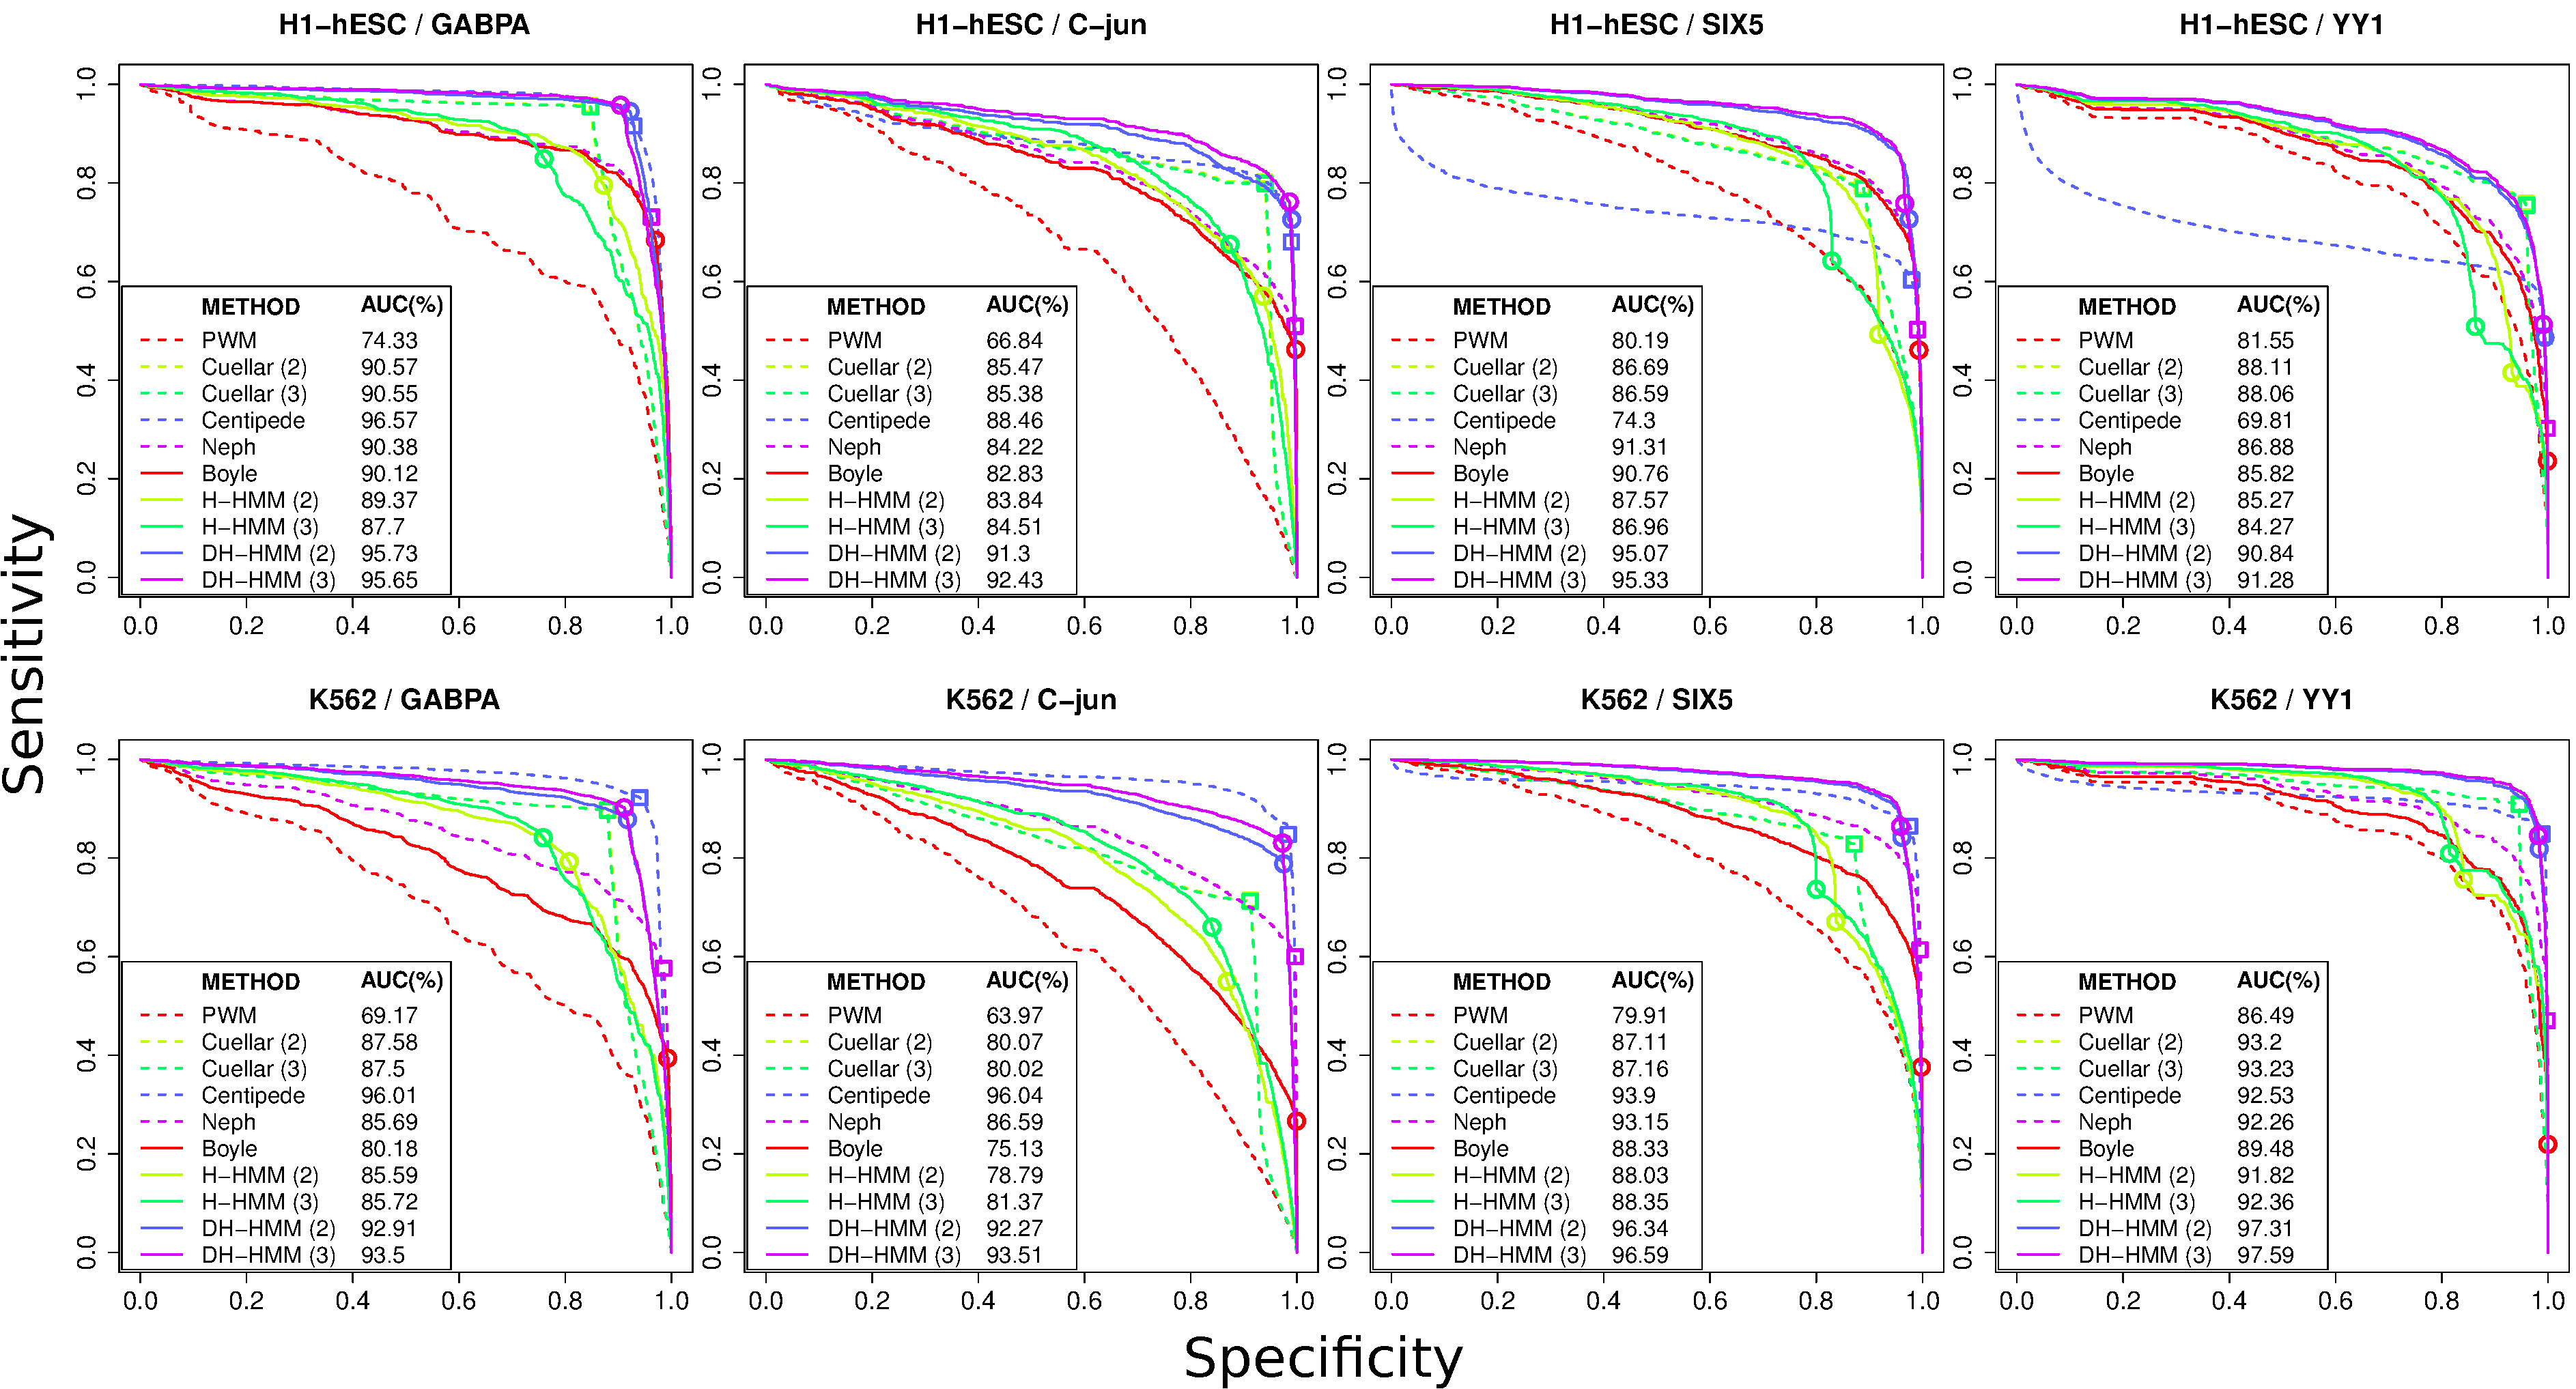
\includegraphics[width=0.99\textwidth]{Figs/ROC.pdf}
\caption{{\color{red} ROC-like} curves for a selection of TFs created when applying the methods to data from the cell types H1-hESC and K562.}
\label{fig:roc}
\end{figure*}

\begin{table}[t]
\vspace{0.0cm}
\begin{center}
\caption{Friedman-Nemenyi hypothesis test results on sensitivity, specificity and AUC. The asterisk and the cross, respectively, mean that the method in the column outperformed the method in the row with significance levels of 0.05 and 0.1.}
\label{tab:friedman.nemenyi}
  \begin{tabularx}{0.45\textwidth}{lrccccccccc}
  & & \rotatebox{90}{DH-HMM (3)} & \rotatebox{90}{DH-HMM (2)} & \rotatebox{90}{Centipede} & \rotatebox{90}{Neph} & \rotatebox{90}{Cuellar (2)} & \rotatebox{90}{Cuellar (3)} & \rotatebox{90}{H-HMM (3)} & \rotatebox{90}{H-HMM (2)} & \rotatebox{90}{Boyle} \\
  \hline
    \multirow{9}{*}{\begin{sideways}\textbf{Sensitivity}\end{sideways}}
    & Cuellar (2) &     &     &     &     &     &     &     &     &     \\
    & Cuellar (3) &     &     &     &     &     &     &     &     &     \\
    & DH-HMM (3)  &     &     &     &     &     &     &     &     &     \\
    & Centipede   &     &     &     &     &     &     &     &     &     \\
    & DH-HMM (2)  &     &     &     &     & $*$ & $*$ &     &     &     \\
    & H-HMM (3)   & $+$ &     &     &     & $*$ & $*$ &     &     &     \\
    & H-HMM (2)   & $*$ & $*$ & $*$ &     & $*$ & $*$ & $*$ &     &     \\
    & Neph        & $*$ & $*$ & $*$ &     & $*$ & $*$ & $*$ &     &     \\
    & Boyle       & $*$ & $*$ & $*$ &     & $*$ & $*$ & $*$ & $*$ &     \\
  \hline
    \multirow{9}{*}{\begin{sideways}\textbf{Specificity}\end{sideways}}
    & Boyle       &     &     &     &     &     &     &     &     &     \\
    & Neph        &     &     &     &     &     &     &     &     &     \\
    & DH-HMM (2)  &     &     &     & $+$ &     &     &     &     & $*$ \\
    & Centipede   &     &     &     & $*$ &     &     &     &     & $*$ \\
    & DH-HMM (3)  &     &     &     & $*$ &     &     &     &     & $*$ \\
    & Cuellar (2) & $*$ & $*$ & $*$ & $*$ &     &     &     &     & $*$ \\
    & H-HMM (2)   & $*$ & $*$ & $*$ & $*$ &     &     &     &     & $*$ \\
    & Cuellar (3) & $*$ & $*$ & $*$ & $*$ &     &     &     &     & $*$ \\
    & H-HMM (3)   & $*$ & $*$ & $*$ & $*$ & $*$ &     &     & $+$ & $*$ \\
  \hline
    \multirow{9}{*}{\begin{sideways}\textbf{AUC}\end{sideways}}
    & DH-HMM (3)  &     &     &     &     &     &     &     &     &     \\
    & DH-HMM (2)  &     &     &     &     &     &     &     &     &     \\
    & Centipede   & $*$ & $*$ &     &     &     &     &     &     &     \\
    & Neph        & $*$ & $*$ &     &     &     &     &     &     &     \\
    & Cuellar (2) & $*$ & $*$ &     &     &     &     &     &     &     \\
    & Cuellar (3) & $*$ & $*$ &     &     &     &     &     &     &     \\
    & H-HMM (3)   & $*$ & $*$ & $*$ & $*$ & $+$ &     &     &     &     \\
    & H-HMM (2)   & $*$ & $*$ & $*$ & $*$ & $*$ & $*$ &     &     &     \\
    & Boyle       & $*$ & $*$ & $*$ & $*$ & $*$ & $*$ &     &     &     \\
  \hline
  \end{tabularx}
\end{center}
\vspace{-1.0cm}
\end{table}

\subsection{Spatial Specificity {\color{red} and DHS Coverage} of Segmentation Approaches}
\label{sec:spatial.specificity}

Next, we evaluated the spatial specificity~\citep{wilbanks2010}, i.e. the distance
of all predicted regions to the center of their recognized active TFBSs. Note that
this comparison is only made on segmentation-based methods (Boyle, Neph and HMM-based
methods), as site-centric methods always have an `ideal' spatial specificity
since they use sequence information. The Fig.~\ref{fig:boxplot} shows the resulting
distribution of distances for all evaluated TFs. Overall, DH-HMMs had better spatial
specificity (lowest distance of footprints to the center of active TFBSs) than all
other methods (Mann-Whitney-Wilcoxon of equal distance distributions was rejected
with $p$-value $\leq 10^{-5}$). On the other hand, the H-HMMs presented large distances
than all other methods ($p$-value $\leq 10^{-5}$). This is again explained by the lower
resolution of the ChIP-seq to indicate chromatin structure in comparison to the DHS
signal. These results indicate that DH-HMMs improve Boyle and Neph methods upon the
detection of the exact location of TFBSs. {\color{red} Lastly, we evaluated footprints statistics inside DHS sites. Footprints from DH-HMM cover $98.67\%$ of DHS sites, while footprints predicted by Boyle and Neph method cover only $30.34\%$ and $45.22\%$ of DHS sites. An inspection of the DNase-seq read coverage indicates that both Boyle and Neph methods fail to identify footprints in DHS sites with low to average read counts. See Supplementary Section~3.8 for further details.}

\begin{figure}[t]
\centering
     \includegraphics[width=0.33\textwidth]{Boxplot.eps}
%     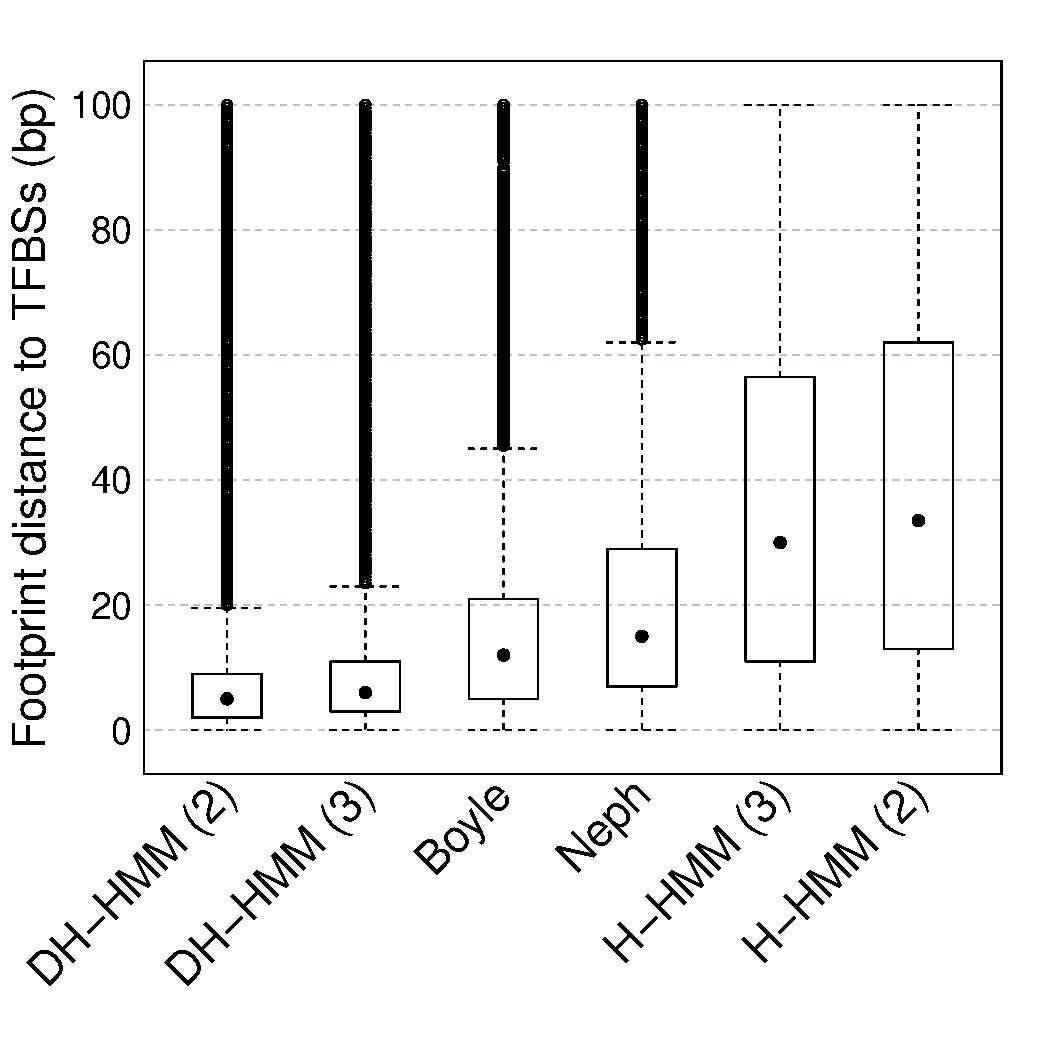
\includegraphics[width=0.33\textwidth]{Figs/Boxplot.pdf}
\caption{Distribution of the distances from genomic positions predicted by segmentation-based methods to the center of the predicted active TFBSs. Results correspond to the absolute distances over all TFs using data from H1-hESC and K562 cell types.}
\label{fig:boxplot}
\end{figure}

\section{Discussion}
\label{sec:discussion}

Methods for detection of active TFBSs can be categorized in two main classes:
site-centric (Cuellar and Centipede) and segmentation-based (Boyle, Neph and
HMMs). Site-centric approaches require the identification of all MPBSs of a
given TF to classify them as active or inactive. One advantage of the latter
methods is that they have an ideal spatial specificity. On the other
hand, they require sequence binding affinity information (PWM) of the TFs to
be known {\color{red}\emph{a priori}}. On the other hand, segmentation-based approaches can be
used for \emph{de novo} motif detection. Indeed, previous studies have shown
that footprints allowed the automatic creation of high-sensitivity TF
models~\citep{kulakovskiy2009} and the discovery of hundreds of novel
motifs~\citep{neph2012a}. Such studies would benefit from segmentation-based
methods with good spatial specificity. Moreover, segmentation-based methods
tend to reduce computational complexity, as they decrease drastically (1-2$\%$)
the genomic space used for motif detection.
{\color{red} However, it is important to mention that the interpretation of such
reduced genomic space would still require knowledge of proteins' binding sequence affinity.}

While Centipede obtained good AUC results, the method's performance was too
dependent on regularization parameters. Moreover, for large input files (TFs
with a large number of PWM hits) the method required up to 6/core days of computing
and 65GB of memory on a single TF and cellular condition. The
most computational expensive segmentation method, DH-HMM, requires 9 days/core for
predicting footprints and active binding sites over all 500 TFs from JASPAR in one
cell type.

Another important aspect is the proposed combined use of DHS and histone
modifications shapes around the TFBSs. Cuellar method is based on obtaining
read counts around the TFBSs. Clearly, such method can not take the local
shape profiles into account. For example, it can not distinguish the DHS peaks
with the footprint signals and would detect any TFBS inside a region with high
DHS levels as the regions indicated in Fig.~\ref{fig:hmm}A. Indeed, our experimental
results confirm the poor specificity of the method. While Centipede used the
local profiles of the DHS signal, it used simple read count statistics for the
histone modification signals. Therefore, it is unable to detect the valley shapes indicated in
Fig.~\ref{fig:hmm}A. Not surprisingly, no improvements were possible with the use
of histone modifications using Centipede, as indicated in~\cite{pique2011}. The
DH-HMM model could indeed show improved results by using the local profiles of DHS and histone modification signals. {\color{red} Moreover, DH-HMM footprints cover a higher percentage of DHS regions than other segmentation-based methods}. 

Recent studies have also indicated that the histone modification profiles centered on DHS
sites can be clustered and these clusters can also have asymmetric shapes,
where there is lower evidence of histone marks downstream or upstream of the DHS.
We have also tested variants of the DH-HMM to capture such asymmetric signals,
but no significant improvement was obtained. As show in Supplementary Fig.~5,
the slope signals have high values changes even on low histone modification values and are
responsible for the correct characterization of such asymmetric peaks. Lastly,
the HMMs displayed robustness in the training/evaluation on distinct cell types.
This indicates that no further training of the HMMs and time intensive manual
annotation of genomic regions are required. This is achieved by addressing both
within- and between-dataset variability with our normalization pipeline.

\section{Final Remarks}
\label{sec:final.remarks}

This paper presents a novel approach to combine the spatial profiles of DHS (DNase-seq)
and histone modifications (ChIP-seq) to predict cell type-specific active TFBSs.
Moreover, we perform a large evaluation of all competing methods over two cell
types and a large validation with 83 TF ChIP-seq datasets. We could show that
the HMM model combining both DHS and histone modification data presents a good
trade-off between sensitivity and specificity in relation to all compared methods.
Furthermore, the method was robust when trained and evaluated in distinct cell
types and has no further parameterization requirements. This study also provides
all footprint predictions and validation data forming the first benchmarking data
set for footprinting analyses. The accumulation of further epigenetic data
and more detailed biological experiments will pose new methodological challenges
to the field. The analysis of a cell type after a differentiation steps or response
stimuli would indicate detailed changes in transcriptional landscape. 

\section*{Acknowledgements}

We would like to thank Pablo A. Jaskowiak, Sonja Haenzelmann, Manuel Allhoff, {\color{red}Joseph Kuo,}
Terry Furey and Shane Neph for providing predictions and sharing code and
the anonymous referees for relevant suggestions.
\paragraph{Funding\textcolon}
This work was supported by the Interdisciplinary Center for Clinical Research
(IZKF Aachen), RWTH Aachen University Medical School, Aachen, Germany; and Brazilian research
agencies: FACEPE and CNPq.

%\bibliographystyle{natbib}
%\bibliography{document}

\begin{thebibliography}{}

\bibitem[{Arvey, A. \emph{et al.}}(2012){Arvey, A. \emph{et al.}}]{arvey2012}
{Arvey, A. \emph{et al.}} (2012).
\newblock {Sequence and chromatin determinants of cell-type-specific
  transcription factor binding}.
\newblock {\em Genome Research\/}, {\bf 22}(9), 1723--1734.

\bibitem[{Bell, O. \emph{et al.}}(2011){Bell, O. \emph{et al.}}]{bell2011}
{Bell, O. \emph{et al.}} (2011).
\newblock Determinants and dynamics of genome accessibility.
\newblock {\em Nat Rev Genet\/}, {\bf 12}(8), 554--564.

\bibitem[{Boyle, A. P. \emph{et al.}}(2008){Boyle, A. P. \emph{et
  al.}}]{boyle2008b}
{Boyle, A. P. \emph{et al.}} (2008).
\newblock F-seq: a feature density estimator for high-throughput sequence tags.
\newblock {\em Bioinformatics\/}, {\bf 24}(21), 2537--2538.

\bibitem[{Boyle, A. P. \emph{et al.}}(2011){Boyle, A. P. \emph{et
  al.}}]{boyle2011}
{Boyle, A. P. \emph{et al.}} (2011).
\newblock {High-resolution genome-wide in vivo footprinting of diverse
  transcription factors in human cells}.
\newblock {\em Genome Research\/}, {\bf 21}(3), 456--464.

\bibitem[{Cock, P. J. A. \emph{et al.}}(2009){Cock, P. J. A. \emph{et
  al.}}]{cock2009}
{Cock, P. J. A. \emph{et al.}} (2009).
\newblock {Biopython: freely available Python tools for computational molecular
  biology and bioinformatics}.
\newblock {\em Bioinformatics\/}, {\bf 25}(11), 1422--1423.

\bibitem[{Crawford, G. E. \emph{et al.}}(2006){Crawford, G. E. \emph{et
  al.}}]{crawford2006b}
{Crawford, G. E. \emph{et al.}} (2006).
\newblock {Genome-wide mapping of DNase hypersensitive sites using massively
  parallel signature sequencing (MPSS)}.
\newblock {\em Genome Research\/}, {\bf 16}(1), 123--131.

\bibitem[{Cuellar-Partida, G. \emph{et al.}}(2012){Cuellar-Partida, G. \emph{et
  al.}}]{cuellar2012}
{Cuellar-Partida, G. \emph{et al.}} (2012).
\newblock {Epigenetic priors for identifying active transcription factor
  binding sites}.
\newblock {\em Bioinformatics\/}, {\bf 28}(1), 56--62.

\bibitem[{ENCODE Project Consortium}(2012){ENCODE Project
  Consortium}]{encode2012}
{ENCODE Project Consortium} (2012).
\newblock An integrated encyclopedia of {DNA} elements in the human genome.
\newblock {\em Nature\/}, {\bf 489}(7414), 57--74.

\bibitem[{Gusm\~{a}o, E. G. \emph{et al.}}(2012){Gusm\~{a}o, E. G. \emph{et
  al.}}]{gusmao2012}
{Gusm\~{a}o, E. G. \emph{et al.}} (2012).
\newblock Prediction of transcription factor binding sites by integrating dnase
  digestion and histone modification.
\newblock In {\em Proc. of the 7th Brazilian Symposium on Bioinformatics\/},
  Campo Grande, Mato Grosso do Sul, Brazil.

\bibitem[{Hon, G. \emph{et al.}}(2009){Hon, G. \emph{et al.}}]{hon2009}
{Hon, G. \emph{et al.}} (2009).
\newblock {Discovery and Annotation of Functional Chromatin Signatures in the
  Human Genome}.
\newblock {\em PLoS Comput Biol\/}, {\bf 5}(11), e1000566+.

\bibitem[{Kim, J. \emph{et al.}}(2008){Kim, J. \emph{et al.}}]{kim2008}
{Kim, J. \emph{et al.}} (2008).
\newblock An extended transcriptional network for pluripotency of embryonic
  stem cells.
\newblock {\em Cell\/}, {\bf 132}(6), 1049--1061.

\bibitem[{Kulakovskiy, I. V. \emph{et al.}}(2009){Kulakovskiy, I. V. \emph{et
  al.}}]{kulakovskiy2009}
{Kulakovskiy, I. V. \emph{et al.}} (2009).
\newblock Motif discovery and motif finding from genome-mapped {DNase}
  footprint data.
\newblock {\em Bioinformatics\/}, {\bf 25}(18), 2318--2325.

\bibitem[{Kundaje, A. \emph{et al.}}(2012){Kundaje, A. \emph{et
  al.}}]{kundaje2012}
{Kundaje, A. \emph{et al.}} (2012).
\newblock {Ubiquitous heterogeneity and asymmetry of the chromatin environment
  at regulatory elements}.
\newblock {\em Genome Research\/}, {\bf 22}(9), 1735--1747.

\bibitem[{Landt, S. G. \emph{et al.}}(2012){Landt, S. G. \emph{et
  al.}}]{landt2012}
{Landt, S. G. \emph{et al.}} (2012).
\newblock {ChIP-seq guidelines and practices of the ENCODE and modENCODE
  consortia}.
\newblock {\em Genome Research\/}, {\bf 22}(9), 1813--1831.

\bibitem[Madden(1978)Madden]{madden1978}
Madden, H.~H. (1978).
\newblock {Comments on the Savitzky-Golay convolution method for least-squares
  fit smoothing and differentiation of digital data}.
\newblock {\em Anal.Chem.}, {\bf 50}, 1383--1386.

\bibitem[{Maston, G. A. \emph{et al.}}(2006){Maston, G. A. \emph{et
  al.}}]{maston2006}
{Maston, G. A. \emph{et al.}} (2006).
\newblock {Transcriptional Regulatory Elements in the Human Genome}.
\newblock {\em Annual Review of Genomics and Human Genetics\/}, {\bf 7}(1),
  29--59.

\bibitem[{Mathelier, A. \emph{et al.}}(2014){Mathelier, A. \emph{et
  al.}}]{mathelier2014}
{Mathelier, A. \emph{et al.}} (2014).
\newblock {JASPAR} 2014: an extensively expanded and updated open-access
  database of transcription factor binding profiles.
\newblock {\em Nucleic Acids Research\/}, {\bf 42}(D1), D142--D147.

\bibitem[{Matys, V. \emph{et al.}}(2006){Matys, V. \emph{et al.}}]{matys2006}
{Matys, V. \emph{et al.}} (2006).
\newblock {TRANSFAC and its module TRANSCompel: transcriptional gene regulation
  in eukaryotes}.
\newblock {\em Nucleic acids research\/}, {\bf 34}(Database issue), D108--D110.

\bibitem[{Natarajan, A. \emph{et al.}}(2012){Natarajan, A. \emph{et
  al.}}]{natarajan2012}
{Natarajan, A. \emph{et al.}} (2012).
\newblock {Predicting cell-type-specific gene expression from regions of open
  chromatin}.
\newblock {\em Genome Research\/}, {\bf 22}(9), 1711--1722.

\bibitem[{Neph, S. \emph{et al.}}(2012){Neph, S. \emph{et al.}}]{neph2012a}
{Neph, S. \emph{et al.}} (2012).
\newblock {An expansive human regulatory lexicon encoded in transcription
  factor footprints}.
\newblock {\em Nature\/}, {\bf 489}(7414), 83--90.

\bibitem[{Ouyang, Z. \emph{et al.}}(2009){Ouyang, Z. \emph{et
  al.}}]{ouyang2009}
{Ouyang, Z. \emph{et al.}} (2009).
\newblock {ChIP}-seq of transcription factors predicts absolute and
  differential gene expression in embryonic stem cells.
\newblock {\em Proceedings of the National Academy of Sciences\/}, {\bf
  106}(51), 21521--21526.

\bibitem[{Pedregosa, F. \emph{et al.}}(2011){Pedregosa, F. \emph{et
  al.}}]{pedregosa2011}
{Pedregosa, F. \emph{et al.}} (2011).
\newblock Scikit-learn: Machine learning in {P}ython.
\newblock {\em Journal of Machine Learning Research\/}, {\bf 12}, 2825--2830.

\bibitem[{Pique-Regi, R. \emph{et al.}}(2011){Pique-Regi, R. \emph{et
  al.}}]{pique2011}
{Pique-Regi, R. \emph{et al.}} (2011).
\newblock {Accurate inference of transcription factor binding from DNA sequence
  and chromatin accessibility data}.
\newblock {\em Genome Research\/}, {\bf 21}(3), 447--455.

\bibitem[Rabiner(1989)Rabiner]{rabiner1989}
Rabiner, L.~R. (1989).
\newblock {A tutorial on hidden Markov models and selected applications in
  speech recognition}.
\newblock {\em Proceedings of the IEEE\/}, {\bf 77}(2), 257--286.

\bibitem[Robasky and Bulyk(2011)Robasky and Bulyk]{robasky2011}
Robasky, K. and Bulyk, M.~L. (2011).
\newblock {UniPROBE}, update 2011: expanded content and search tools in the
  online database of protein-binding microarray data on {protein-DNA}
  interactions.
\newblock {\em Nucleic acids research\/}, {\bf 39}(Database issue).

\bibitem[Stormo(2000)Stormo]{stormo2000}
Stormo, G.~D. (2000).
\newblock {DNA binding sites: representation and discovery}.
\newblock {\em Bioinformatics\/}, {\bf 16}(1), 16--23.

\bibitem[{Thurman, R. E. \emph{et al.}}(2012){Thurman, R. E. \emph{et
  al.}}]{thurman2012}
{Thurman, R. E. \emph{et al.}} (2012).
\newblock {The accessible chromatin landscape of the human genome}.
\newblock {\em Nature\/}, {\bf 489}(7414), 75--82.

\bibitem[{Wang, J. \emph{et al.}}(2013){Wang, J. \emph{et al.}}]{wang2013}
{Wang, J. \emph{et al.}} (2013).
\newblock Factorbook.org: a wiki-based database for transcription
  factor-binding data generated by the {ENCODE} consortium.
\newblock {\em Nucleic Acids Research\/}, {\bf 41}(D1), D171--D176.

\bibitem[{Whitington, T. \emph{et al.}}(2009){Whitington, T. \emph{et
  al.}}]{whitington2009}
{Whitington, T. \emph{et al.}} (2009).
\newblock {High-throughput chromatin information enables accurate
  tissue-specific prediction of transcription factor binding sites}.
\newblock {\em Nucleic Acids Research\/}, {\bf 37}(1), 14--25.

\bibitem[Wilbanks and Facciotti(2010)Wilbanks and Facciotti]{wilbanks2010}
Wilbanks, E.~G. and Facciotti, M.~T. (2010).
\newblock Evaluation of algorithm performance in {ChIP}-seq peak detection.
\newblock {\em PloS one\/}, {\bf 5}(7), e11471+.

\bibitem[{Wilczynski, B. \emph{et al.}}(2009){Wilczynski, B. \emph{et
  al.}}]{wilczynski2009}
{Wilczynski, B. \emph{et al.}} (2009).
\newblock Finding evolutionarily conserved cis-regulatory modules with a
  universal set of motifs.
\newblock {\em BMC bioinformatics\/}, {\bf 10}(1), 82+.

\bibitem[{Won, K. J. \emph{et al.}}(2010){Won, K. J. \emph{et al.}}]{won2010}
{Won, K. J. \emph{et al.}} (2010).
\newblock {Genome-wide prediction of transcription factor binding sites using
  an integrated model}.
\newblock {\em Genome Biology\/}, {\bf 11}(1), R7+.

\bibitem[{Zhang, Y. \emph{et al.}}(2008){Zhang, Y. \emph{et al.}}]{zhang2008}
{Zhang, Y. \emph{et al.}} (2008).
\newblock {Model-based analysis of ChIP-Seq (MACS)}.
\newblock {\em Genome biology\/}, {\bf 9}(9), R137+.

\end{thebibliography}

\end{document}


